%%%%%%%%%%%%%%%%%%%%%%% file template.tex %%%%%%%%%%%%%%%%%%%%%%%%%
%
% This is a general template file for the LaTeX package SVJour3
% for Springer journals.          Springer Heidelberg 2010/09/16
%
% Copy it to a new file with a new name and use it as the basis
% for your article. Delete % signs as needed.
%
% This template includes a few options for different layouts and
% content for various journals. Please consult a previous issue of
% your journal as needed.
%
%%%%%%%%%%%%%%%%%%%%%%%%%%%%%%%%%%%%%%%%%%%%%%%%%%%%%%%%%%%%%%%%%%%
%

\RequirePackage{fix-cm}
%
\documentclass{svjour3}                     % onecolumn (standard format)
%\documentclass[smallcondensed]{svjour3}     % onecolumn (ditto)
%\documentclass[smallextended]{svjour3}       % onecolumn (second format)
%\documentclass[twocolumn]{svjour3}          % twocolumn
%
\smartqed  % flush right qed marks, e.g. at end of proof
%
\usepackage{graphicx}
\usepackage{amsmath}
\usepackage{enumitem}
\usepackage{marvosym}
\usepackage{appendix}
\usepackage{xcolor}
%
% \usepackage{mathptmx}      % use Times fonts if available on your TeX system
%
% insert here the call for the packages your document requires
%\usepackage{latexsym}
% etc.
%
% please place your own definitions here and don't use \def but
% \newcommand{}{}
%
% Insert the name of "your journal" with
% \journalname{myjournal}
%
\begin{document}

\title{RealPot: an immersive virtual pottery system with handheld haptic devices
%\thanks{Grants or other notes
%about the article that should go on the front page should be
%placed here. General acknowledgments should be placed at the end of the article.}
}
%\subtitle{Do you have a subtitle?  \\ If so, write it here

%\titlerunning{Short form of title}        % if too long for running head

\author{Zihan Gao		\and
		Huiqiang Wang	\and
        Guangsheng Feng	\and
		Fangfang Guo 	\and
		Hongwu Lv 		\and
		Bingyang Li
}

%\authorrunning{Short form of author list} % if too long for running head

\institute{Zihan Gao \and Huiqiang Wang(\Letter) \and Guangsheng Feng \and \\Fangfang Guo \and Hongwu Lv \and Bingyang Li \at
            College of Computer Science and Technology, Harbin Engineering University, Harbin, China\\
            \email{wanghuiqiang@hrbeu.edu.cn}\\
            Telephone:+86-0451-8258-9605\\
            Fax:+86-0451-8258-9605
	\and	Zihan Gao \at
			\email{gao\_zihan@126.com}
    \and	Guangsheng Feng \at
			\email{ica@hrbeu.edu.cn}
   \and		Fangfang Guo \at
			\email{guofangfang@hrbeu.edu.cn}
   \and		Hongwu Lv \at
			\email{lvhongwu@hrbeu.edu.cn}
   \and		Bingyang Li \at
			\email{libingyang@hrbeu.edu.cn}
}

\date{Received: date / Accepted: date}
% The correct dates will be entered by the editor


\maketitle

\begin{abstract}

We present \textbf{RealPot}, an immersive virtual pottery system with haptic feedback for pottery simulation training using hand-held motion controllers.
%
Our system consists of two major components: an automatic mesh generator and an interactive model editor.
%
The mesh generator can procedurally generate realistic clay meshes by adding Perlin Noise.
%
With the interactive pottery model editor, the user can shape the virtual clay intuitively with a series of bimanual interactions.
%
{\color{blue}
Based on real-life pottery, a high realism pottery creation workflow was developed and a haptic model was proposed.
%
Our user study investigated how haptic fidelity can impact usability in virtual pottery, and compared our system with a representative work of barehand-based virtual pottery systems.
%
The results of our study reveal that haptic fidelity significantly affects performance and user experience.
%
In addition, the results indicate that our system offers significantly accuracy, presence and usability compared with barehand-based virtual pottery experience.
}

%Insert your abstract here. Include keywords, PACS and mathematical
%subject classification numbers as needed.
\keywords{Virtual pottery \and Natural user interfaces \and Mesh deformation \and Haptic feedback}
% \PACS{PACS code1 \and PACS code2 \and more}
% \subclass{MSC code1 \and MSC code2 \and more}
\end{abstract}

{\color{blue}

%%% Introduction
%With the purpose in simulation training,

\section{Introduction}
\label{sec:intro}

With the increasing realism provided by advancing technologies, virtual reality (VR) has shown great potential for art and design.
%
In the last two decades, virtual pottery has become an interesting research topic in computer aided design (CAD), which provides novel modeling experience in VR.
%
Compared with general-purpose professional modeling tools such as Maya \cite{website:maya} and 3ds Max \cite{website:3dmax}, virtual pottery systems usually have easy-to-use user interfaces, specifically designed for pottery creation simulation.
%
Although researchers have explored this topic by proposing a variety of virtual pottery systems, it is not completely clear how fidelity can impact usability and user performance in virtual pottery systems.

%% motivation
A number of virtual pottery systems have been developed in the recent past.
%
Among the existing works, using depth cameras as input devices has become a trend in recent years \cite{ramani2015gesture,murugappan2013handy,han2014virtual,gao2018digiclay} , where users can create virtual pots with barehand-based interactions.
%
In these systems, users can deform the mesh intuitively with bare hands, the hand gestures and postures are captured by cameras and then mapped to mesh operations.
% limitation
Although barehand-based interactions are simple for novice users, jitters and occlusions from depth cameras may sometimes lead to imprecise inputs, which hinders work efficiency and user experience.
%
In terms of \textit{display fidelity} (the objective degree of exactness with which real-world sensory stimuli are reproduced), immersion and haptic feedback have not been considered in the existing works.
%
Furthermore, although with the purpose of pottery simulation training, existing works only considered the deformation phase, overlooking the complete workflow in real-life pottery.
%
In addition, due to unchangeable deformation parameters, which cannot be interactively tuned by users, creativities offered by these systems are often limited.

%% goals
Considering the importance of fidelity and limitations in the existing works, we designed RealPot, an immersive virtual pottery system with haptic feedback that allows users to design pottery models using hand-held motion controllers.
%
There are three major design goals for RealPot:
%
(1) design an immersive experience for virtual pottery with realistic haptic feedback,
%
(2) implement a realistic workflow for pottery simulation training, 
%
and (3) add helpful features to support creativities for virtual pottery design, such as parameter control, undo and redo etc. 

To overcome the imprecise inputs from depth cameras, we used wireless handheld motion controllers as input devices, which can not only provide input precision, but also increase display fidelity from haptic aspects.
%
As for visual aspects, we used a head-mounted display in our system rather than a monitor to create a first-person immersive experience, with which the user can adjust viewport interactively based on head movement.
%
Aiming for achieving a higher realism for pottery simulation training, we implemented a complete workflow for virtual pottery system, which is based on real-life pottery creation process.
%
To support more creativities, some functionalities were integrated in our system, which allowed more possibilities of deformation effects, and provided convenience for users.

%% contributions
The main contributions of our works are:
% display fidelity
(1) We added realism to the existing virtual pottery works by developing an immersive system with a realistic simulation of haptic sensations, and investigated how haptic fidelity impact the usability in virtual pottery.
% interaction fidelity
(2) We expanded virtual pottery simulation by implementing a complete workflow based on real-life pottery, and integrated functionalities to support more creativities.

The paper is structured as follows:
Section 2 introduces the related work about virtual pottery.
The technical details of the system are demonstrated in Section 3.
In Section 4, we set up two comparative user studies.
Finally, the discussions for the system are given in Section 5, followed by the conclusions in Section 6.
%%%

}

\section{Related Work}
\label{sec:related}

\subsection{Bimanual Interactions}
\label{sec:bimanual}
Bimanual interactions have been a popular research field, which can accomplish a variety of tasks in both physical and virtual environments.
In terms of mechanisms, bimanual interactions can be classified into two categories: barehand-based interactions and instrument-based interactions.

There are a great number of research efforts \cite{walter2014cuenesics,cui2016exploration,ramani2015gesture,murugappan2013handy,han2014virtual} on barehand-based interactions using depth camera such as Kinect, Leap Motion, etc.
Cuenestics \cite{walter2014cuenesics} is a design space for hand-gesture based mid-air selection techniques using a depth camera Kinect, where users can select contents on interactive public displays with their gesture inputs.
Cui et al. \cite{cui2016exploration} proposed a modeling system with natural freehand interactions using a Leap Motion controller, allowing users to grab and manipulate objects with one or two hands intuitively.
While these works provide accessibility to users, they have some common limitations: The inputs are inaccurate due to many factors such as lighting condition, occlusion, etc., which could handicap work efficiency and cause user frustration.
In addition, these methods do not provide haptic feedback, which hinders the realistic feel for users in the interaction process.

Unlike barehand-based interactions, instrument-based interactions provide more control precision, haptic feedback and unambiguity.
Surface Drawing \cite{schkolne2001surface} is a system for creating organic 3D shapes using tangible tools such as data gloves, where users can define strokes with the path of hands wearing data gloves.
Hinckley et al. \cite{hinckley1998two} investigated two-handed virtual manipulation with a point design of a prop-based system, which allows users to view a cross section of a brain with interface props.
These works have a common issue that the usage of these instruments is limited to a lab context that very few users can access.
%
With the commercialization of gaming devices, some motion controllers such as Wii Remote and HTC Vive have become accessible to consumers, which are also used in scientific studies for 3D user interfaces \cite{wingcrave2010wii,niehorster2017accuracy}.
%
In our project, HTC Vive system is used in our system, which provides precision, haptic feedback and well accessed by consumers.

\subsection{Art and Design Tools in VR}
\label{sec:art}
Virtual reality has shown great potential for art and design, which not only provides immersive and intuitive interfaces for user, but also creates new art medium, new art form and novel experience \cite{laviola20113d}.

CavePainting \cite{keefe2001cavepainting} is a 3D artistic medium in a fully immersive VE, which enables artists to create spatial paintings with physical props and gestures. Agrawala et al. \cite{agrawala19953d} developed an interface for painting on polygon meshes using a 6DOF space tracker, which provides a natural force feedback for painting, allowing users to place colors on meshes intuitively. MAI Painting Brush++ \cite{otsuki2017brush} is a brush device for virtual painting of 3D virtual objects, where users could take a physical object in the real world and apply virtual paint to it with visual and haptic feedback.
Virtual Clay \cite{mcdonnell2001virtual} is a sculpture framework based on subdivision solids and physics-based modeling, which is equipped with natural, haptic based interaction, providing users with a realistic sculpting experience. Sheng et al. \cite{sheng2006interface} proposed an interface for virtual 3D sculpting, which uses camera-based motion tracking technology to track passive markers on the fingers and prop, enabling users to apply operations such as deforming, smoothing, pasting and extruding.

To leverage the novel experience brought by VR, the setup of our system is based on a VE, where users can enjoy the creation process in an immersive way.

\subsection{Virtual Pottery Systems}
\label{sec:virtual}

%Unlike some sculpting systems mentioned above, virtual pottery systems allow rotational symmetry, and much easier for novice users.
%Qp \cite{koutsoudis2009qp} was a tool for generating 3D pottery models, which can produce a collection of random 3D ancient Greek vessels.
%Based on number-theoretic techniques, Kumar et al. \cite{kumar2011wheel} presented a system for creating digital potteries including thick-walled potteries as well, which resembles pottery works in real life.
%While these systems can generate heterogeneous pottery models efficiently, their user interfaces are limited to traditional keyboard and mouse input, which are not helpful for training users to understand the pottery creation process.

A number of virtual pottery systems have been developed in the recent past.
One of the earliest virtual pottery systems is CHINA \cite{korida1997interactive}, where users can create pottery works wearing digital gloves and stereoscopic glasses.
Systems such as \cite{koutsoudis2009qp} and \cite{kumar2011wheel} can generate heterogeneous pottery models instantly, where users need to input parameters using keyboard and mouse input.
Ramani et al. proposed a series of freehand systems based on depth cameras, where point cloud data is analyzed to extract user design intent \cite{ramani2014zpots,ramani2015gesture,ramani2016extracting}.
Handy-Potter \cite{murugappan2013handy} is a rapid 3D creation tool, which tracks user skeletons with Kinect, enabling users to create potteries in several seconds based on the trails of both hands.
Han and Han \cite{han2014virtual} presented an audiovisual interface, where pottery shapes deformed by hand motions are translated into musical sound.
In AR Pottery \cite{han2007ar}, augmented reality has been applied to pottery design, with which users can deform a virtual pottery using a marker held by hand.

Although the interfaces provided by these systems are not difficult to learn, some realistic features are ignored and the workflow is oversimplified, which might not be helpful in the context of simulation training.
%
In order to add realism to virtual pottery based on the existing works, our system provides a much {\color{blue} more} realistic workflow and experience, which allows users to manipulate virtual clay through various two-handed spatial interactions, helping novice users to understand and learn real-life pottery skills in a VE.


\section{Interactive Modeling for Virtual Pottery}
\label{sec:interactive}


\subsection{System Overview}
\label{sec:overview}
RealPot is an interactive modeling system for virtual pottery based on handheld haptic devices in VR.
Users can create pottery in our system with bimanual inputs, deforming the virtual clay in realtime.
RealPot can export the mesh data as an OBJ file when a pottery work is finished, which can be used in 3D printing.
Our system provides a simulation training environment in virtual worlds, allowing novice users and children to learn pottery skills interactively.

%%%Fig%%% results
\begin{figure}
\includegraphics[width=\textwidth]{fig1}
\caption{A user is using our system to create virtual pots.}
\label{fig:demo}
\end{figure}

\subsubsection{System Architecture}
\label{sec:architecture}

The system architecture is demonstrated in Figure \ref{fig:arc}. When the mesh generator generates a clay mesh, users can start to interact with the mesh with handheld haptic devices. The deformation manager is the core component of the mesh editor, which will deform the clay, sending information to haptic manager and UI manager. The haptic manager will send pulses to motion controller as haptic feedback, and the UI manager will update the UI elements, sending to the head-mounted display via the rendering engine. Once the creation is done, the mesh IO manager will convert the meshes into OBJ files and save them.

%%%Fig%%% architecture
\begin{figure*}
\includegraphics[width=\textwidth]{fig2}
\caption{The system architecture of RealPot.}
\label{fig:arc}
\end{figure*}



\subsubsection{Workflow}
\label{sec:workflow}
In real life, the pottery creation process on a pottery wheel is called \textit{throwing}, where a ball of clay is placed in the center of a turntable wheel-head, and shaped by a potter.
{\color{blue}Some interactions used in RealPot simulate the operations in real-life pottery.}
To illustrate the pipeline of pottery creation in our system, an example workflow using RealPot is described as follows.

When a user starts to use RealPot, a realistic clay mesh is automatically generated with Perlin noise (Figure \ref{fig:workflow}a, Section \ref{sec:generation}). 
Similar to the operation in reality, the user first need to use both hands to make the irregular clay shape into perfect rotational symmetry, which is called \textit{centering} (Figure \ref{fig:workflow}b, Section \ref{sec:rotational}).
The user can control the thickness of the clay (i.e. \textit{opening}) by pressing down the clay to create a hollow in the clay (Figure \ref{fig:workflow}c), 
and then draw up the walls with two hands moving up together (i.e. \textit{pulling}), controlling the height of the clay (Figure \ref{fig:workflow}d, Section \ref{sec:thickness}).
The system not only allows mesh deforming (Figure \ref{fig:workflow}e, Section \ref{sec:deformation}) with different deformation range parameters but also mesh smoothing (Figure \ref{fig:workflow}f, Section \ref{sec:smoothing}), where the user can remove sharp features in the pot to get an ideal shape.
After the creation process is finished, the user can export the pottery model as an OBJ file, which can be used for 3D printing.

%%%Fig%%% workflow
\begin{figure*}
\includegraphics[width=\textwidth]{fig3}
\caption{The workflow in RealPot. (a) The automatically generated clay mesh with Perlin Noise. (b) The mesh is shaped into rotational symmetry by holding both hands. (c) The user controls the thickness of the mesh by pressing down the clay. (d) The user controls the height of the mesh by drawing up the clay wall. (e) The deformation range can be adjusted to get varied deformation effect on different parts. (f) The sharp features on the upper part can be removed by mesh smoothing.}
\label{fig:workflow}
\end{figure*}



\subsection{Mesh Generation}
\label{sec:generation}

Mesh generation is the first step of interactive modeling, and most of virtual pottery systems approximate the initial shape of pottery clay as a primitive cylinder shape \cite{han2007ar,ramani2015gesture,ramani2016extracting}.
Although this approach is simple to implement, it ignores subtle details of clay, whose irregularity needs to be handled first during the creation process in real life.
Unlike the existing virtual pottery systems, RealPot first approximates the initial clay on the pottery wheel as a blending shape of cylinder and semi-ellipsoid, then adds Perlin noises to the basic clay, in order to simulate realistic clay features in reality.

\subsubsection{Basic Clay}

The clay mesh is described as a generalized cylinder, whose resolution can be defined by axis segments $s_{a}$ and height segments $s_{h}$. Given radius $r$ and height $h$, our system can generate primitive mesh of cylinder and semi-ellipsoid respectively (Figure \ref{fig:base}).
For each vertex in the mesh, a $m \times n$ matrix $M$ is used to store radius values, where the number of row $m = s_{h} + 1$ and the number of column $n = s_{a}$ respectively. The base radius $r_{base_{i}}$ of each vertex $\mathbf{v}_{i,j}$ in row $i$ can be calculated as: 

\begin{equation}
r_{base_{i}} = \alpha \cdot \frac{r}{h} \sqrt{h^2 -  h_{i}^2} + (1 - \alpha) \cdot r
\end{equation}
\begin{equation}
h_{i} = i \cdot \frac{h}{m-1}
\end{equation}
where $\alpha$ is a factor controls the shape blending between a cylinder (when $\alpha=0$) and a semi-ellipsoid (when $\alpha=1$) (Figure \ref{fig:base}).

%%%Fig%%% base mesh
\begin{figure*}
\includegraphics[width=\textwidth]{fig4.pdf}
\caption{The basic clay generated by our system, which is a blending shape between a cylinder and a semi-ellipsoid. $\alpha$ is the blending factor which controls the radius on the top.}
\label{fig:base}
\end{figure*}

\subsubsection{Adding Noise}

Although the initial shape of clay can be roughly approximated like a rotational symmetric shape, in real life, the actual clay shape is not regular, whose irregular features needs to be specially treated during the pottery creation process. To simulate the realistic features, randomness is added to the vertices using Perlin Noise \cite{Perlin1985An}, which is a smooth random method proposed by Ken Perlin in 1985.
In our approach, the center positions for each circular section are randomized first, then Perlin Noise is added to the radii for each circular section and individual vertices.

To add noise to the center for each circular section, random parameters $\phi_{i}$ and $\eta_{c_{i}}$ are used to calculate the new center $\mathbf{O}_{i}$:
\begin{equation}
\label{eqn:oi}
\mathbf{O}_{i} = \left[\eta_{c_{i}}cos\phi_{i}, h_{i}, \eta_{c_{i}}sin\phi_{i}\right]^T
\end{equation}
where $\phi_{i} \in [0, 2\pi]$ is a random degree, and $\eta_{c_{i}}$ is a random radius.
Then the new radii $r_{total_{i,j}}$ for each vertex can be computed by getting the sum of $r_{base_{i}}$ and noise values:
\begin{equation}
r_{total_{i,j}} = r_{base_{i}} + \eta_{row_{i}} + \eta_{indv_{i,j}}
\end{equation}
where $\eta_{row_{i}}$ is the radius noise for each circular section, and $\eta_{indv_{i,j}}$ is the individual radius for each vertex (Figure \ref{fig:noise}). The radius value $r_{i,j}$, along with the position $\mathbf{v}_{i,j}$ for each vertex can be computed in the follow equations:
\begin{equation}
r_{i,j} = \left\|
\mathbf{O}_{i} + \left[ r_{total_{i,j}} cos \theta_{j},
0,
r_{total_{i,j}} sin \theta_{j}
\right]^T
\right\| 
\end{equation}

\begin{equation}
\theta_{j} = j \cdot \frac{2\pi}{n}
\end{equation}

\begin{equation}
\label{eqn:v}
\mathbf{v}_{i,j} =
\left[r_{i,j}  cos \theta_{j},
h_{i},
r_{i,j} sin \theta_{j}\right]^T
\end{equation}

%%%Fig%%%
\begin{figure*}
\includegraphics[width=\textwidth]{fig5.pdf}
\caption{To get a noised radius $r_{i,j}$ (green) based on radius $r_{base_{i}}$ (red): (1) Move the center from origin (0,0) to $\mathbf{O}_{i}$. (2) Calculate the sum: $r_{total_{i,j}} = r_{base_{i}} + r_{row_{i}} + r_{indv_{i,j}}$. (3) Find the distance to the origin, which will be the noised radius $r_{i,j}$.}
\label{fig:noise}
\end{figure*}

\subsubsection{Inner Vertices}

To create 3D printing-oriented pottery models, our system needs to generate watertight 3D models with thickness.
To accomplish that, RealPot generates inner and bottom sides based on the outer side mesh. The vertices on inner side can be denoted as:

\begin{equation}
\label{eqn:v'}
\mathbf{v'}_{i,j} 
= \begin{cases}
\begin{bmatrix}
0,h_{i},0
\end{bmatrix}^T & \beta=1
\\
\begin{bmatrix}
r'_{i,j} \cdot cos \theta_{j},
h_{i},
r'_{i,j} \cdot sin \theta_{j}
\end{bmatrix}^T & 0 \le \beta<1
\end{cases}
\end{equation}

\begin{equation}
r'_{i,j} = r_{i,j} - \max(t_{min}, r_{top} \cdot \beta)
\end{equation}
where $\beta$ is the thickness ratio of the clay, whose range is $[0,1]$. In mesh generation phase, the default value of $t$ is 1, which means the clay is a solid shape; in mesh deformation phase, the value of $t$ can be adjusted by users interactively, getting a center-hollowed shape. $t_{min}$ is a predefined value for the minimum thickness, and $r_{top}$ is the largest radius value for the top section, which guarantees equal thickness for each part.
Vertices for inner-bottom and outer-bottom sides will be then generated according to inner-side and outer-side vertices respectively. Finally, a mesh can be generated by constructing triangle faces based on the vertex indices (Figure \ref{fig:mesh}).

%%%Fig%%% Mesh
\begin{figure}
\includegraphics[width=\textwidth]{fig6}
\caption{The meshes generated with our system. (a) A regular mesh without adding Perlin noise. (b) A mesh with Perlin noise, which is more realistic as a clay.}
\label{fig:mesh}
\end{figure}

\subsection{Mesh Editing}
\label{sec:editing}
After observing and analyzing several real-life pottery throwing videos, we put real-life clay operations into 5 categories: (1) rotational symmetry control, (2) thickness control, (3) height control, (4) deformation and (5) smoothing.
{\color{blue} Corresponding to the clay operations above, 5 mesh editing operations are designed in our system, namely, \textit{centering}, \textit{opening}, \textit{pulling}, \textit{shaping} and \textit{smoothing}.}
These operations will be discussed in detail in the following sections.
Since any clay mesh $C$ can be generated from key parameters including height $h$, thickness $t$ and radius matrix $M$, a mesh generation function is constructed: $C =  g(h, t, M)$, which can be used to update the mesh data as well.
In our approach, RealPot first modifies key parameters of the clay according to user interactions, then updates mesh data $C$ in real time based on these parameters using the mesh generation function.

\subsubsection{Rotational Symmetry Control}
\label{sec:rotational}
\textit{Centering} is the first important operation in pottery creation in reality, where people press the ball of clay downward and inward, making the irregular clay into perfect rotational symmetry.
In our system, the user can use two controllers to touch the virtual clay and pull the trigger button to achieve symmetry control (Figure \ref{fig:workflow}b).
The mean radius value of each row in the radius matrix is calculated and then each radius value in matrix needs updating based on the mean radius values:
\begin{equation}
\label{eqn:sym}
r'_{i,j} = 
\lambda \cdot \frac{1}{n}\sum_{k=1}^{n} r_{i,k}
+ (1 - \lambda) \cdot r_{i,j}
\end{equation}
where $\lambda \in [0,1]$ is a damping factor controlling the rate of symmetry.
The effect of rotational symmetry control is illustrated in Figure \ref{fig:symmetry}.

%		Fig:Symmetry
\begin{figure*}
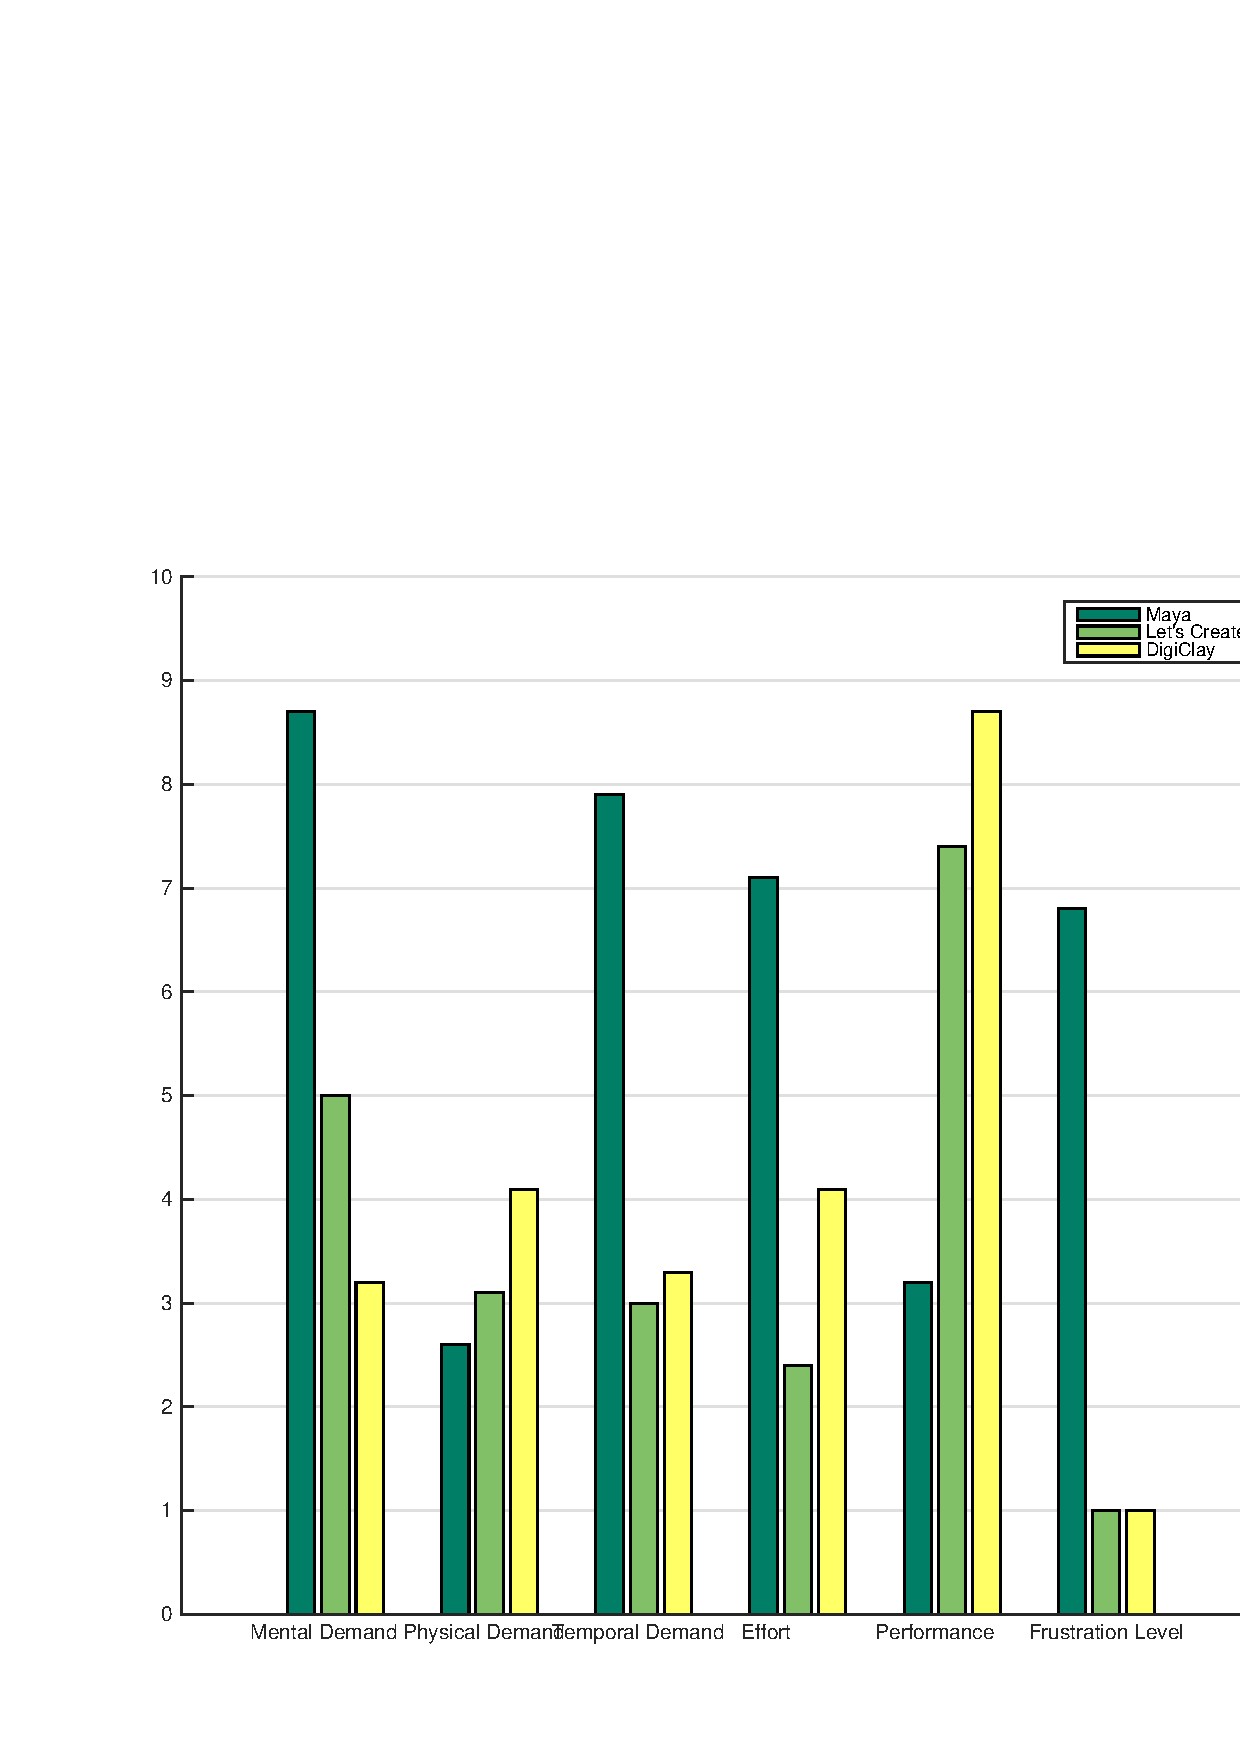
\includegraphics[width=\textwidth]{fig7.pdf}
\caption{Rotational symmetry control. The blue curve is the noised circular section at height $h_{i}$, and the green curve is a circle with the average radius $\bar r_{i}$. Let $\Delta r_{i,j}$ be the difference between $r_{i,j}$ and $\bar r_{i}$, then multiplied by the damping factor $\lambda$. New radius be calculated : $r'_{i, j} = r_{i,j} - \lambda\Delta r_{i}$, which is identical to Equation (\ref{eqn:sym}). }
\label{fig:symmetry}
\end{figure*}

\subsubsection{Thickness and Height Control}
\label{sec:thickness}
\textit{Opening} (thickness control) and \textit{pulling} (height control) are basic clay operations in pottery throwing process which are done by applying force to clay with both hands. The thickness can be adjusted by pushing down the top center part of the clay, making a centered hollow into the clay (Figure \ref{fig:workflow}c). The height can be adjusted by both hands drawing up and shaping the walls (Figure \ref{fig:workflow}d).
Let $\Delta y$ be the mean of $\Delta y_{l}$ and $\Delta y_{r}$, which are left and right vertical hand movement distance respectively. New height $h'$ and new thickness ratio $\beta'$ can be calculated in the following equations:
\begin{equation}
\Delta y = (\Delta y_{l} + \Delta y_{r})/2
\end{equation}
\begin{equation}
h' = h_{0} + \Delta y * \gamma
\end{equation}
\begin{equation}
\beta' = \beta_{0} + \Delta y/ h
\end{equation}
where $h_{0}$ and $\beta_{0}$ are initial height and thickness ratio values before deformation respectively; $\gamma$ is a damping factor for height. And the new mesh data will be recomputed using new values $h'$ and $\beta'$.

\subsubsection{Mesh Deformation}
\label{sec:deformation}
In this section, interactive deformation in our system will be discussed. According to \cite{botsch2010polygon}, this topic is challenging since complex mathematical formulations (1) have to be hidden behind an intuitive user interface and (2) have to be implemented in a sufficiently efficient and robust manner to allow for interactive applications.

In our approach, a cylindrical coordinate system is used to specify the position for each vertex, where y-axis is the reference axis. For any point $P$ in the coordinate system, we use$(\rho, \phi, y)$ to denote the position, where the radial distance $\rho$ is the Euclidean distance from the y-axis to the point P; $\phi$ is the azimuth; $y$ is the height of point P from xz-plane.
Due to rotational symmetry in virtual pottery, RealPot modifies the $\rho$ for each vertex while keeping $\phi$ and $y$ constant. Thus, the deformation problem is turned into how to calculate the new radius $\rho'_{i,j}$ based on hand movement:
\begin{equation}
\rho'_{i,j} = \rho_{i,j} + \Delta \rho_{i,j}
\end{equation}

% base on 3D cursor radial dist
Let $(x_{0},y_{0},z_{0})$ be the initial 3D cursor position at time $t_{0}$ when the deformation starts, and we can calculate the initial radial distance of the 3D cursor from y-axis: $\rho_{0} = \sqrt{x_{0}^2 + z_{0}^2}$. The new 3D cursor position at time $t_{1}$ is $(x_{1},y_{1},z_{1})$, and the new radial distance is $\rho_{t} = \sqrt{x_{1}^2 + z_{1}^2}$.
% vertical dist
When the user presses the trigger button on the controller while the 3D cursor touches the mesh, the vertical distance $d_{i,j}$ between the 3D cursor and each vertex $\mathbf{v}_{i,j}$ can be computed as:
\begin{equation}
d_{i,j} = |y_{0} - y_{i,j}|
\end{equation}
where $y_{i,j}$ is the height of $\mathbf{v}_{i,j}$.
In our system, outer range $R_{O}$ and inner range $R_{I}$ are two key parameters affecting deformation effect, which divides the mesh into three regions: fixed region, moving region and deformation region (Figure \ref{fig:deform}a).
The fixed region will keep constant during the deformation, where $d_{i,j} > R_{O}$; the moving region will follow the movement of the 3D cursor, where $d_{i,j} < R_{I}$; and the deformation region will be affected based on the weights, where $R_{I} < d_{i,j} < R_{O}$.
%The deformation region should deform in an intuitive and smooth manner.
Note that when $R_{I} = 0$, the deformation will go in a smooth way; when $R_{I} = R_{O}$, it is possible to create sharp features on the clay:
\begin{equation}
\Delta r_{i,j} = \begin{cases}
\rho_{t} - \rho_{0} &  d_{i,j} < R_{I} \\
0 &  d_{i,j} > R_{O} \\
(\rho_{t} - \rho_{0}) \cdot w_{i,j} &  R_{I} < d_{i,j} < R_{O}
\end{cases}
\end{equation}

%get weight from falloff curve
A falloff curve is needed in order to get smooth deformation effect when calculating weights: $w_{i,j} = f(t)$, where $t = (d_{i,j} - R_{I}) / (R_{O} - R_{I})$.
There are many ways to select a smooth falloff functions for the weights, which needs to satisfy these additional requirements: (i) f(0) = 1 , (ii) f(1) = 0 and (iii) f'(0) = f'(1) = 0.
In order to efficiently calculate the weights, we choose a cubic polynomial function $f(t) = at^3 + bt^2 + ct + d$ as the weight falloff function, we have:
\begin{equation}
\begin{aligned}
\label{equation:falloff}
f(0) = 1 \\
f(1) = 0 \\ 
f'(0) = 0 \\
f'(1) = 0
\end{aligned}
\end{equation}
we can find the solution from Equation (\ref{equation:falloff}), where 
$a = 2, b = -3, c = 0, d = 1$. Therefore, the expression of the falloff function is $f(t) = 2t^3 - 3t^2 + 1$ (Figure \ref{fig:deform}b).

%%%Fig%%%
\begin{figure*}
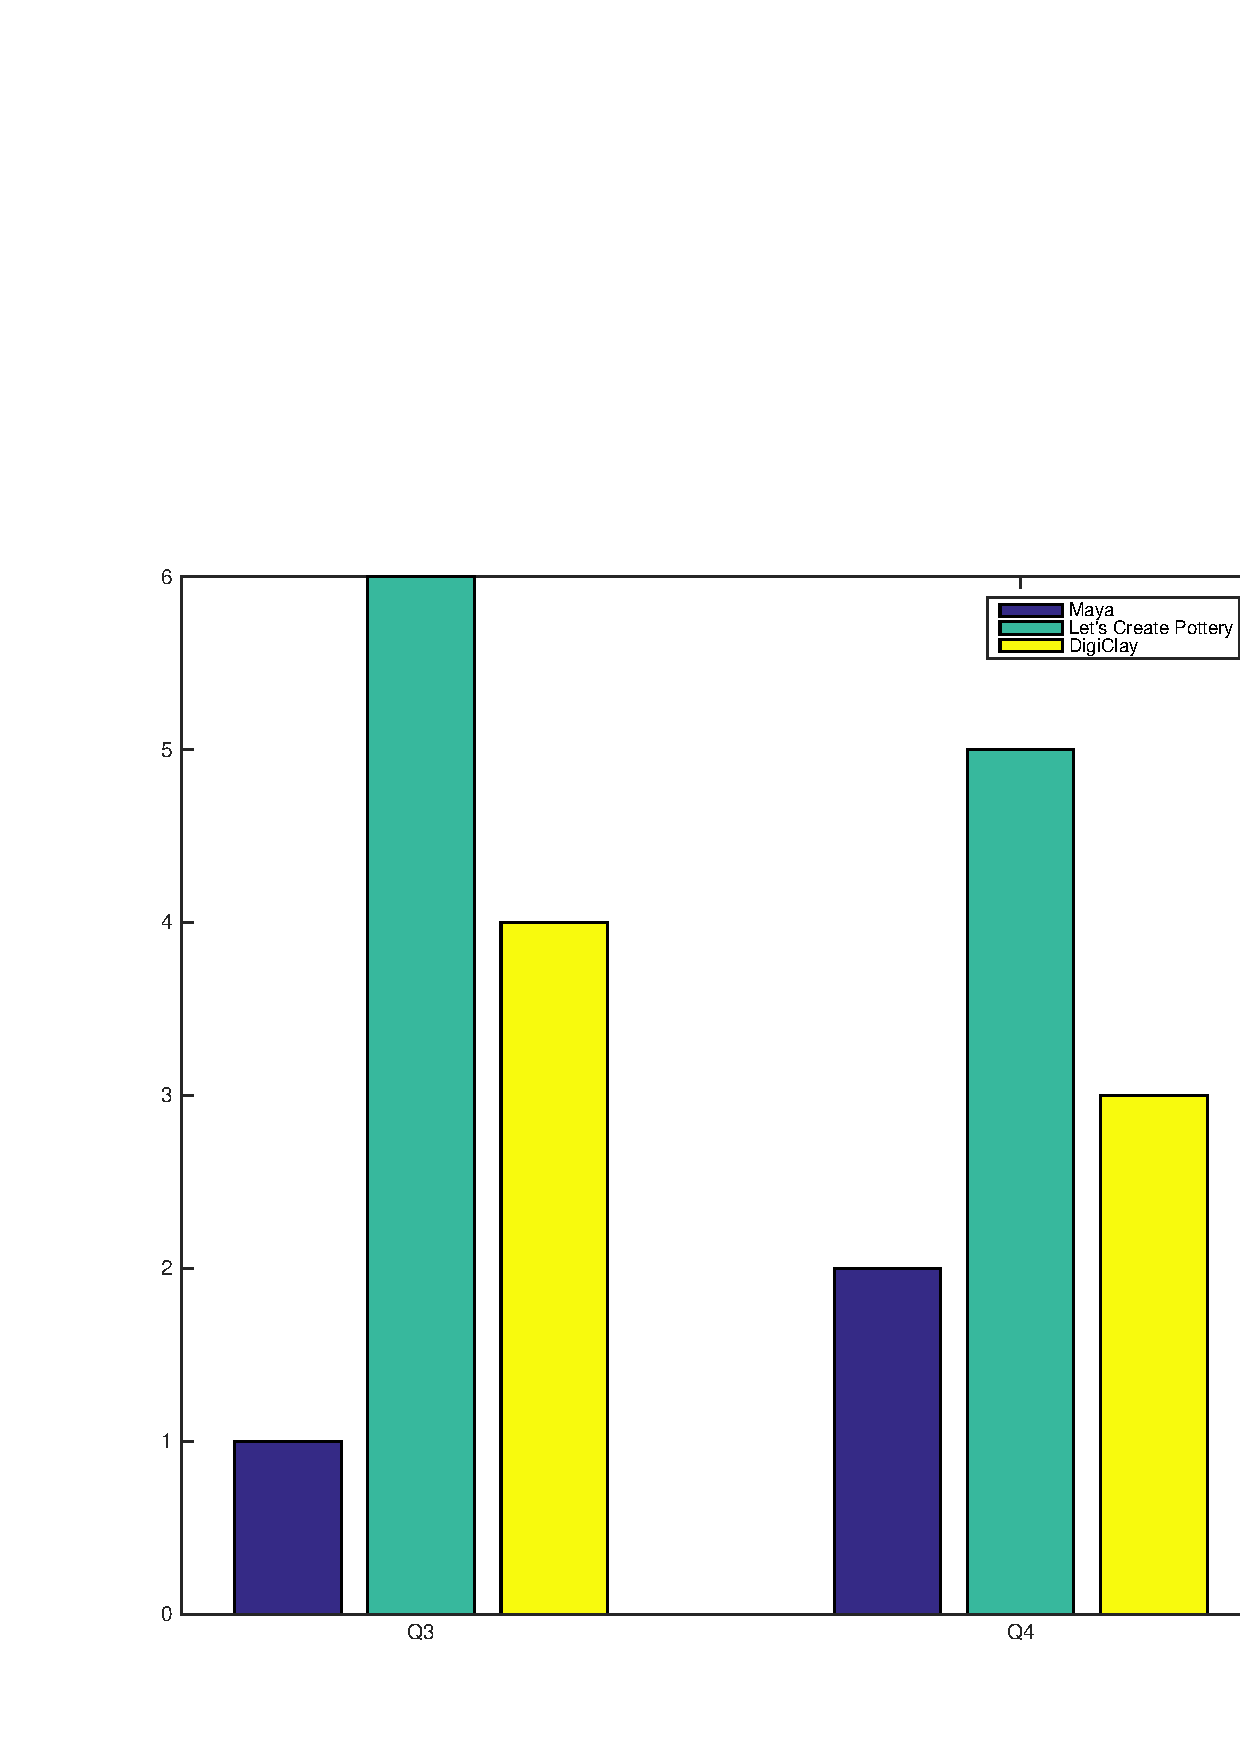
\includegraphics[width=\textwidth]{fig8.pdf}
\caption{(a) The concentric circles represent the 3D cursor, and $R_{I}$ and $R_{O}$ define the inner range and outer range respectively. $d_{i,j}$ is the vertical distance between a vertex $\mathbf{v}_{i,j}$ in the deformation region and the 3D cursor, which is used for calculating weight parameter : $t = (d_{i,j} - R_{I}) / (R_{O} - R_{I})$. (b) A cubic polynomial function $f(t) = 2t^3 - 3t^2 + 1, t \in [0,1]$ is used as the falloff curve for calculating the weight $w_{i,j}$. }
\label{fig:deform}
\end{figure*}

\subsubsection{Mesh Smoothing}
\label{sec:smoothing}
As mentioned above, it is possible to create sharp features upon the clay mesh during the deformation process. In order to remove unwanted sharp features, our system uses Laplacian smoothing:
\begin{equation}
r'_{i,j} = 
\omega  \frac{1}{N} 
\sum_{k=1}^N r_{k}
+ (1 - \omega)  r_{i,j}
\end{equation}
where $N$ is the number of adjacent vertices of $\mathbf{v}_{i,j}$; $\omega \in [0,1]$ is a factor controlling the smoothing effect.
Only the vertices within the range of the 3D cursor $R_{O}$ will be affected.
As a result, users can control the 3D cursor position and adjust the outer range $R_{O}$ of the 3D cursor to apply smoothing on specific areas interactively on the mesh.


{\color{blue}

\subsection{Haptic Feedback Model}
\label{sec:haptic}

Haptic feedback in a 3D user interface is a powerful tool in developing more effective, efficient and immersive experiences \cite{laviola20173d}.
However, little work has been done on haptic feedback in the existing virtual pottery systems, due to their intrinsic barehand-based interaction mechanisms.
To design a realistic experience for our virtual pottery system, we first analyzed the sensations in real life pottery, then proposed a haptic model based on the analysis.


\subsubsection{Analysis of the sensation in real life pottery}

In real life pottery, users can perceive forces from hands and fingers when performing various operations on clays.
From these forces, users can obtain information such as clay shape, smoothness, etc.
In general, the haptic feedback from clays can be classified into two categories based on the type of forces: (1) friction forces and (2) reaction forces.
When a user softly touches the clay without exerting too much force, he/she can perceive the \textit{friction forces} on fingers or hands since the clay is rotating.
In addition, when a user exerts force large enough to deform the clay, \textit{reaction forces} are generated in the opposite direction to the movement.
By applying the mechanisms that simulate the both forces to the five mesh editing operations described in Section \ref{sec:editing}, we can realize a virtual pottery system with realistic haptic feedback.
The mechanisms will be described in detail in the following subsections.


\subsubsection{Friction Forces Simulation}

In this subsection, we describe a model to calculate the friction force, which is generated when the user touches the surface of the rotating clay.
For calculation efficiency, we assumed the friction type as kinetic friction, which is a force that opposes the relative motion between moving surfaces.
The frictional force $F_{f}$ can be calculated by the following equation:

\begin{equation}
F_{f} = \mu \cdot F_{n}
\end{equation}
where $\mu$ is the coefficient of friction between clay and hand, and $F_{n}$ is the normal force exerted on the clay surface. According to the equation, the friction force is proportional to the normal force exerted on the clay surface.

Since all the mesh editing operations in our system can be performed using handheld controllers, the trigger value is used as the input of normal force.
The trigger value ranges from 0 to 1, which indicates how much has the user pulled the trigger button.
In HTC Vive handheld controllers, haptic feedback is generated by the built-in vibrators. In every rendering frame, the intensity value can be sent to each controller.
The haptic pulse intensity based on friction is calculated as:

\begin{equation}
k_{f} = k_{0} + \epsilon \cdot k_{\mu}
\end{equation}
where $k_{0}$ is the minimum friction intensity when user just touches the clay, and $\epsilon \in [0,1]$ is analog value of the trigger button. $k_{\mu}$ is the predefined intensity coefficient based on the coefficient of friction $\mu$.


\subsubsection{Reaction Forces Simulation}

In a process of real pottery creation, when a user exerts force to deform the clay by pushing or pulling, in return, the clay exerts reaction force on the hand.
According to Newton's Third Law of classical mechanics, the forces between the hand and the clay exist in equal magnitude and opposite direction.
Hence, the reaction force $\mathbf{F}_{r}$ can be calculated based on the movement of the controller using Newton's Second Law:

\begin{equation}
\mathbf{F}_{r} = -\mathbf{F}_{c} = -m \frac{\mathrm{d} \mathbf{v}}{\mathrm{d} t}
\end{equation}
where $\mathbf{F}_{c}$ is the force exerted by the controller on the clay; $\mathbf{v}$ is the velocity of the controller; $m$ is the mass of the controller.
The reaction haptic intensity $k_{r}$ in each frame can be calculated based on the consecutive controller positions in the last three frames:

\begin{equation}
k_{r} = k_{\nu} \cdot \|\mathbf{v} - \mathbf{v}'\| = k_{\nu} \cdot \|(\mathbf{x}-\mathbf{x}') - (\mathbf{x}'-\mathbf{x}'')\| = k_{\nu} \cdot \|\mathbf{x}-2\mathbf{x}'+\mathbf{x}''\|
\end{equation}
where $k_{\nu}$ is a predefined coefficient; $\mathbf{x}$ is the controller position in the current frame; $\mathbf{x}'$ and $\mathbf{x}''$ are the consecutive controller positions in the last two frames.
The total haptic intensity is the sum of the friction haptic component and the reaction haptic component:

\begin{equation}
k_{\sigma} = k_{r} + k_{f}
\end{equation}

By providing haptic feedback based on $k_{\sigma}$, we can implement the sensation based on clay deformation.
In addition, our system can provide visual cues on both bubbles, which will be highlighted when touching the clay (Figure \ref{fig:highlight}).


%%%Fig%%% Highlight
\begin{figure}
\includegraphics[width=\textwidth]{fig10}
\caption{The visual and haptic feedback when user touches the clay. (a) The normal state of the 3D cursor when it is not touching the clay. (b) The highlight state of the 3D cursor when a user has touched the clay, with a haptic pulse to the corresponding hand.}
\label{fig:highlight}
\end{figure}
}
%In addition, visual feedback

\subsection{Interactions}
\label{sec:interactions}

%the system in a virtual studio - pottery wheel
RealPot is designed as a pottery studio built in a VE.
In our implementation, we use a HTC Vive VR system \cite{website:vive}, which includes a head-mounted display (HMD) and two hand-held controllers to track user head orientation and bimanual movements (Figure \ref{fig:ui}).
%immersion
%head tracking
The HMD uses head tracking to create a human-centric rather than a computer-determined point of view, and the two hand-held controller allows user to manipulate the mesh in a natural and realistic way.
The goal of our system is not only to provide realistic experience in pottery creation, but also to provide convenient operations to improve the efficiency of pottery design. 
Jacob et al. \cite{Jacob2008Reality} summarized that the designer's goal should be to allow the user to perform realistic tasks realistically, to provide additional non real-world functionality, and to use analogies for these commands whenever possible.
As a result, our system offers several operations in VR for pottery design.
The buttons on the controllers are assigned with different functionalities for convenience. The user can control deformation parameters with dominant hand, and perform undo and redo with non-dominant hand.
The mesh reset button and mesh export button are designed on the side of the pottery wheel, as they are not frequently used during the work process, which could prevent user errors.
There are three main operations supported by our system:

\paragraph{Parameter Adjustment}
Parameter adjustment allows the user to control the deformation effect.
The user can adjust the outer range $R_{O}$ by pressing the upper and lower part of the pad on the controller, which controls the influence area. The inner range $R_{I}$ can be adjusted by pressing left and right part of the pad. This function is designed to activate using dominant hand since parameter adjustment is frequently used during the process. Users can adjust the inner and outer ranges while get immediate visual feedback from the size of the sphere.

\paragraph{Undo/Redo}
RealPot allows users to revert changes using undo and redo, which provides automatic support for recovery from user errors and misunderstandings as well as a mechanism for exploring alternatives.
Undo and redo are important interactive features whose absence seriously degrades the usability of an interactive program \cite{choudhary1995general}.
%Our system provides capturing the state of the program before user actions.
Undo and redo buttons are placed on non-dominant hand controller, which allows user to revert changes made on the clay easily.

\paragraph{Mesh Reset/Export}
Mesh reset allows users to start over from the beginning.
Whenever a user touches this button, the generated mesh on the pottery wheel will be reset to initial state. Since the shape is randomized, the user can keep getting a new shape until she is satisfied with the shape.
When the virtual pot is finished, the mesh should be able to export for further use. Our system can encode the mesh data into an OBJ file, and save the file on the disk. The exported OBJ file can be used for 3D printing.


\begin{figure*}
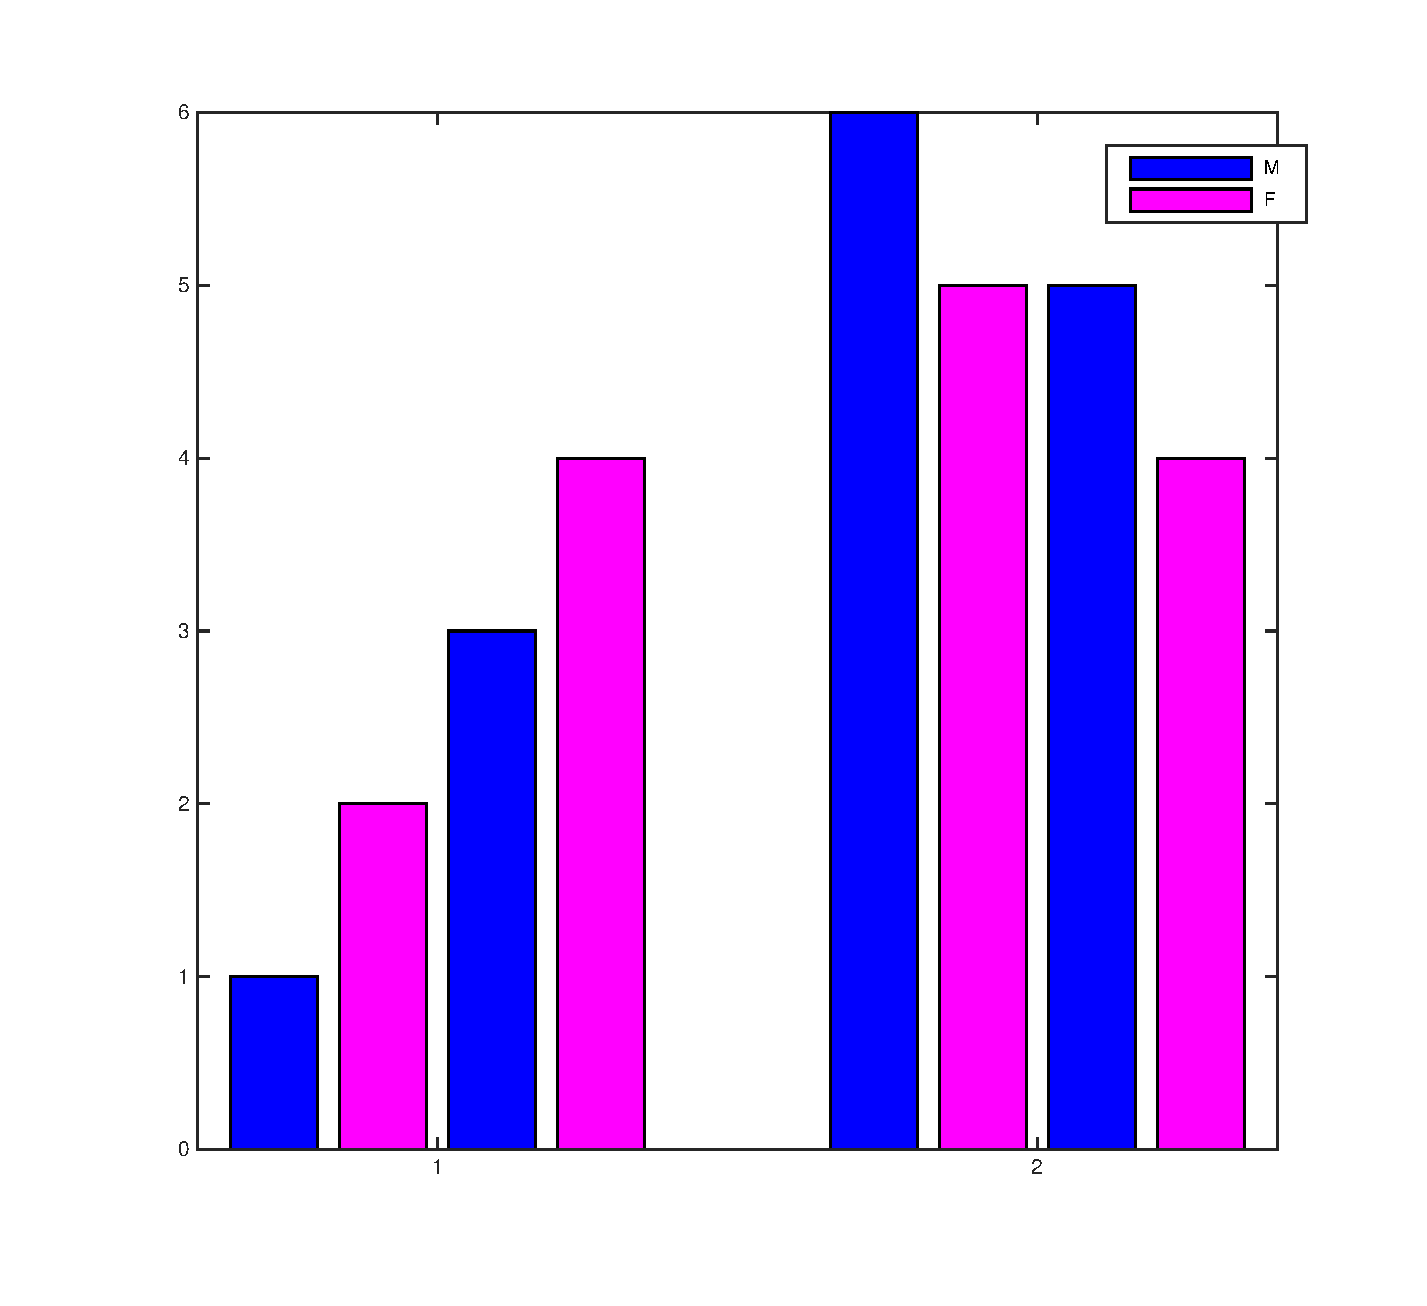
\includegraphics[width=\textwidth]{fig9}
\caption{The user interface of our system. (a) The pottery wheel in the virtual space. (b) The controller button configuration of RealPot. (c) The button layout of left controller pad. (d) The button layout of right controller pad.}
\label{fig:ui}
\end{figure*}


\subsection{System Configurations}
\label{sec:config}

%platform
We have implemented RealPot using Unity3D \cite{website:unity} game engine. RealPot is built on an HTC Vive VR system with a PC (2.10 GHz Dual Core CPU, 16 GB RAM and NVIDIA GeForce GTX 1080 graphics card) running 64-bit Windows 10 Professional.

In order to get performance statistics of the mesh generator, RealPot is tested to generate 4 models with different resolutions.
Based on the common size of clay placed on pottery wheels, we set the height 0.2 units with the radius 0.15 units.
The outer range of the handles is set to 0.2 units, and the inner range is set to 0 to get smooth deformation effect as the process begins. The centering parameter $\lambda$, height parameter $\gamma$ and smoothing parameter $\omega$ are set to 0.5, 0.4 and 0.7 respectively, in order to get a more realistic deformation via damping.
%tables
Table \ref{tab:stats} demonstrates statistics based on different mesh solutions. Higher resolution requires more generation time, since more vertices and triangles need to be calculated and assigned. In general, the performance of mesh generator is sufficient for the requirement in RealPot.

\begin{table}
% table caption is above the table
\caption{Statistics for different axis and height segments.}
\label{tab:stats}       % Give a unique label
% For LaTeX tables use
\begin{tabular}{lllll}
\hline\noalign{\smallskip}
Axis Segments & Height Segments & Vertices & Triangles & Generation Time (ms)\\
\noalign{\smallskip}\hline\noalign{\smallskip}
60 & 100 & 12242 & 24120 & 21.48 \\
60 & 200 & 24242 & 48120 & 41.53 \\
120 & 100 & 24482 & 48240 & 42.02 \\
120 & 200 & 48482 & 96240 & 101.00 \\
\noalign{\smallskip}\hline
\end{tabular}
\end{table}

%%%Fig%%% pots
\begin{figure*}
\includegraphics[width=\textwidth]{fig11}
\caption{The virtual pots designed by our system, which are real-time rendered in Unity3D.}
\label{fig:pots}
\end{figure*}


{\color{blue}


\section{User Studies}
\label{sec:study}

\subsection{User Study 1: Haptic Fidelity Comparison}

The goal of the first user study was to investigate how different haptic feedback levels can impact user experience in our system. 
%
Although McMahan et al. found that display fidelity significantly affect performance in virtual environments \cite{mcmahan2012evaluating}, their experiments only focused on the visual aspects, in which haptic display fidelity was not considered.
%
To increase experimental control and reduce confounds, we adopted a systematic approach that utilized an HTC Vive virtual system to control for confounds while investigating haptic fidelity.
%
As the independent variable, haptic fidelity had three levels (\textit{None}, \textit{Basic} and \textit{Advanced}) and was varied within subjects.
%
The presentation order of the three levels was counterbalanced between subjects.


\subsubsection{Apparatus}
In order to evaluate different levels of display fidelity, we used an HTC Vive virtual system, which contains a HMD and two wireless handheld motion controllers.
%HMD
The HMD has a resolution of 2160 x 1200 (1080 x 1200 per eye) and a refresh rate of 90 Hz.
%controllers
The wireless motion controllers can generate pulses to provide users with haptic feedback, which also have multiple input methods including a track pad, grip buttons and a dual-stage trigger.

\subsubsection{Participants}
% participants
30 participants were participated in our user study, 19 males and 11 females, whose age ranged from 23 to 41 years (mean = 27.07, std = 4.59). 13 of the subjects had experience using VR systems (43.3\%); 6 of the subjects had amateur pottery throwing experience in real life (20\%).

\subsubsection{Experimental Design and Procedure}

Each participant was required to fill out a background survey, which collected general demographic information and real pottery expertise and VR experience.
%2. 
In the next phase, each participant experienced a quick VR training for five minutes.
Since it is possible that the participants were first time users to virtual reality, that subjective evaluation might be influenced by "wow-factors".
Hence, we hoped VR familiarity could eliminate these situations.

\textbf{Task} Given a pottery model in the virtual environment as the target shape, the subjects were asked to create a pot from irregular generated meshes using RealPot as close to the target shape as possible.

To control for confounds, the visual feedback is temporarily disabled during user study 1.
The participants were required to perform the task in three haptic levels, and the order of the three conditions was counterbalanced between subjects:

%3 conditions
\textbf{None}: In this condition, RealPot did not provide any haptic or visual feedback. Users could not receive any haptic sensations when interacting with the virtual clay.

\textbf{Basic}: In this case, RealPot only provided minimum haptic feedback. For example, a haptic pulse will be generated when a cursor touched the virtual clay or a deformation operation was performed.

\textbf{Advanced}: In the advanced haptic model, the system provided dynamic haptic feedback based on our proposed haptic model in Section \ref{sec:haptic}. The haptic intensity depended on how hard the trigger button was pressed and how fast the handheld controllers moved.


\subsubsection{Metrics}

To evaluate the overall performance of the three haptic conditions, we collected metrics related to objective user performance and subjective judgments of usability.
%
For user performance, we measured completion time and accuracy. The accuracy was the correlation coefficient between the user-created shape data and the target shape data.
%
Each participant evaluated the usability in three haptic conditions using a seven-point Likert scale, with 1 being the most negative score, 7 the most positive.

\subsubsection{Study Results}

% time
For completion times, we performed a one-way ANOVA and the results showed haptic fidelity had a significant effect ($F = 26.165, p < 0.0001$).
%
Based on a Tukey HSD post-hoc test, \textit{None} was significantly the most time-consuming condition, while the other two conditions were not significantly different from each other.
% accuracy
For accuracy, another one-way ANOVA showed that haptic fidelity had no significant effects.
% usability
For subjective seven-point Likert scale usability score, we performed a one-way ANOVA and the results showed haptic fidelity had significant effects ($F = 140.170, p < 0.0001$).
%
Post hoc comparison using Tukey HSD test indicated that participants judged \textit{Advanced} (mean = 5.97, std = 0.56) as significantly the best condition while \textit{None} (M = 2.97, 0.72) was judged as significantly the worst condition.

\begin{table}
% table caption is above the table
\caption{Average and standard deviation of user study 1 (upper row: average, bottom row: standard deviation).}
\label{tab:r1}       % Give a unique label
% For LaTeX tables use
\begin{tabular}{llll}
\hline\noalign{\smallskip}
Haptic Fidelity Level & Time & Accuracy & Usability Score\\
\noalign{\smallskip}\hline\noalign{\smallskip}
None & 64.1 & 0.86 & 2.97 \\
 & 4.33 & 0.04 & 0.72 \\\\
Basic & 56.5 & 0.86 & 4.70 \\
 & 5.05 & 0.04 & 0.79 \\\\
Advanced & 56.43 & 0.87 & 5.97 \\
 & 4.75 & 0.04 & 0.56 \\
\noalign{\smallskip}\hline
\end{tabular}
\end{table}


\begin{figure*}
	\includegraphics[width=\textwidth]{fig12.pdf}
	\caption{Results in user study 1. (a) Completion time under each haptic condition. (b) Accuracy under each haptic condition. (c) Usability score under each haptic condition.}
	\label{fig:r1}
\end{figure*}



\subsection{User Study 2: System Usability Comparison}

In user study 2, we wanted to compare the usability of RealPot with existing virtual pottery systems.
%
To compare user experience between instrument-based and barehand-based systems, we used DigiClay \cite{gao2018digiclay} as a representative work of barehand-based virtual pottery systems.
Although these two systems share identical basic functionality, they have different levels of realism.
Compared with DigiClay, our system has higher fidelity, including first-person immersive experience and rich haptic feedback.
\subsubsection{Apparatus}

The two evaluated systems were as follows:

\textbf{RealPot}: Our virtual pottery tool based on a HTC Vive VR system, which had the identical setup in user study 1. The user can shape the virtual clay with bimanual spatial interactions using handheld motion controllers. 

\textbf{DigiClay}: DigiClay is an interactive installation for virtual pottery, where the user can interact with a virtual clay with bare hands.
%monitor
We used a Dell 23.8" LED monitor with a 1920 x 1080 resolution and 60Hz refresh rate as the output device.
%kinect specs
As the input of DigiClay, a motion sensing device Kinect was used, which was composed of a RGB camera and a IR camera both with 640 x 480 resolution and 30 Hz refresh rate.

%PC
The interfaces of the two systems are demonstrated in Figure \ref{fig:sys} respectively, and a comparison of these systems is listed in Table \ref{tab:sys}. 


%%%Fig%%% Sys
\begin{figure*}
\includegraphics[width=\textwidth]{fig13}
\caption{The systems used in our user study. (a) RealPot: the proposed immersive virtual pottery system based on handheld haptic motion controllers (b) DigiClay: a representative of barehand-based virtual pottery systems.}
\label{fig:sys}
\end{figure*}


% For tables use
\begin{table}
% table caption is above the table
\caption{A comparison of the two systems used in our user study.}
\label{tab:sys}       % Give a unique label
% For LaTeX tables use
\begin{tabular}{llllll}
\hline\noalign{\smallskip}
System & Input Method & Head Tracking & Haptic Feedback & Parameter Control \\
\noalign{\smallskip}\hline\noalign{\smallskip}
RealPot & Hand-held Motion Controllers & Yes & Yes & Yes\\
DigiClay & Barehand & No & No & No\\
\noalign{\smallskip}\hline
\end{tabular}
\end{table}


\subsubsection{Participants}
36 participants were participated in user study 2, 23 males and 13 females, whose age ranged from 22 to 33 years (mean = 25.86, std = 2.95, not involved in user study 1). 12 of the subjects are familiar with VR systems (33.3\%) and 7 of the subjects have amateur pottery experience in real life (19.4\%).


\subsubsection{Experimental Design and Procedure}

%1. 
Similar to user study 1, each participant was required to fill out a background survey, which collected general demographic information and real pottery expertise and VR experience.
%2. 
In the next phase, each participant experienced a quick VR training for five minutes to get familiar with VR and remove "wow-factors" influence in the subjective judgments.

After the VR exposure phase, participants proceeded through the two tasks below. The presentation order of the two tasks was counterbalanced between subjects.

\textbf{Task 1} Given a pot model as the target shape, the subjects were asked to create a pot using RealPot as close to the target shape as possible.

\textbf{Task 2} Given a pot model as the target shape, the subjects were asked to create a pot using DigiClay as close to the target shape as possible.

There was a training session before each task, in which the experimenter explained how to interact with the given system and the participant was allowed to practice. After the practice session, participants were instructed to shape the clay according to the target shape as quickly as possible while maintaining high accuracy. Afterwards, the participants were given the usability and presence questionnaires.


\subsubsection{Metrics}
To evaluate the overall performance of the two systems, we collected metrics related to objective user performance and subjective judgments of usability and presence.
For user performance, we measured completion time and accuracy.
The accuracy was the correlation coefficient between the user-created shape data and the target shape data.

For perceptions of presence, we used Slater-Usoh-Steed (SUS) Presence Questionnaire after each trial \cite{slater1994depth}.
To measure the usability of pottery systems, we developed our own usability questionnaire consisting of seven-point Likert-scale items (see Appendix).


\subsubsection{Study Results}

% time
For completion times, we performed a one-way ANOVA and the results showed the two systems had no significant effect.
% accuracy
For accuracy, we performed a one-way ANOVA and the results showed RealPot was significantly more accurate than DigiClay ($F = 13.979, p < 0.0001$). 
% presence
For subjective presence questionnaire, we performed a one-way ANOVA and the results showed different haptic models had a significant effect ($F = 120.598, p < 0.0001$).
% usability
For subjective usability questionnaire, we performed a one-way ANOVA and the results showed different haptic models had a significant effect ($F = 106.609, p < 0.0001$).
% relations
To determine if participants' backgrounds hand any significant effects on our results, we computed Pearson correlation coefficients to assess the relationships between objective metrics and participants' real pottery experience. We found a positive correlation between pottery expertise and completion time ($r = 0.333, p = 0.004$), and a positive correlation between pottery expertise and accuracy ($r = 0.423, p < 0.0001$).

\begin{table}
% table caption is above the table
\caption{Average and standard deviation of user study 2 (upper row: average, bottom row: standard deviation).}
\label{tab:r2}       % Give a unique label
% For LaTeX tables use
\begin{tabular}{lllll}
\hline\noalign{\smallskip}
System & Time & Accuracy & Presence Score & Usability Score\\
\noalign{\smallskip}\hline\noalign{\smallskip}
RealPot 	& 54.44	& 0.86 & 5.81 & 6.08 \\
			& 6.83	& 0.04 & 0.75 & 0.73 \\
\\
DigiClay 	& 54.19	& 0.82 & 3.83 & 4.36 \\
			& 6.35	& 0.03 & 0.77 & 0.68 \\
\noalign{\smallskip}\hline
\end{tabular}
\end{table}

\begin{figure*}
	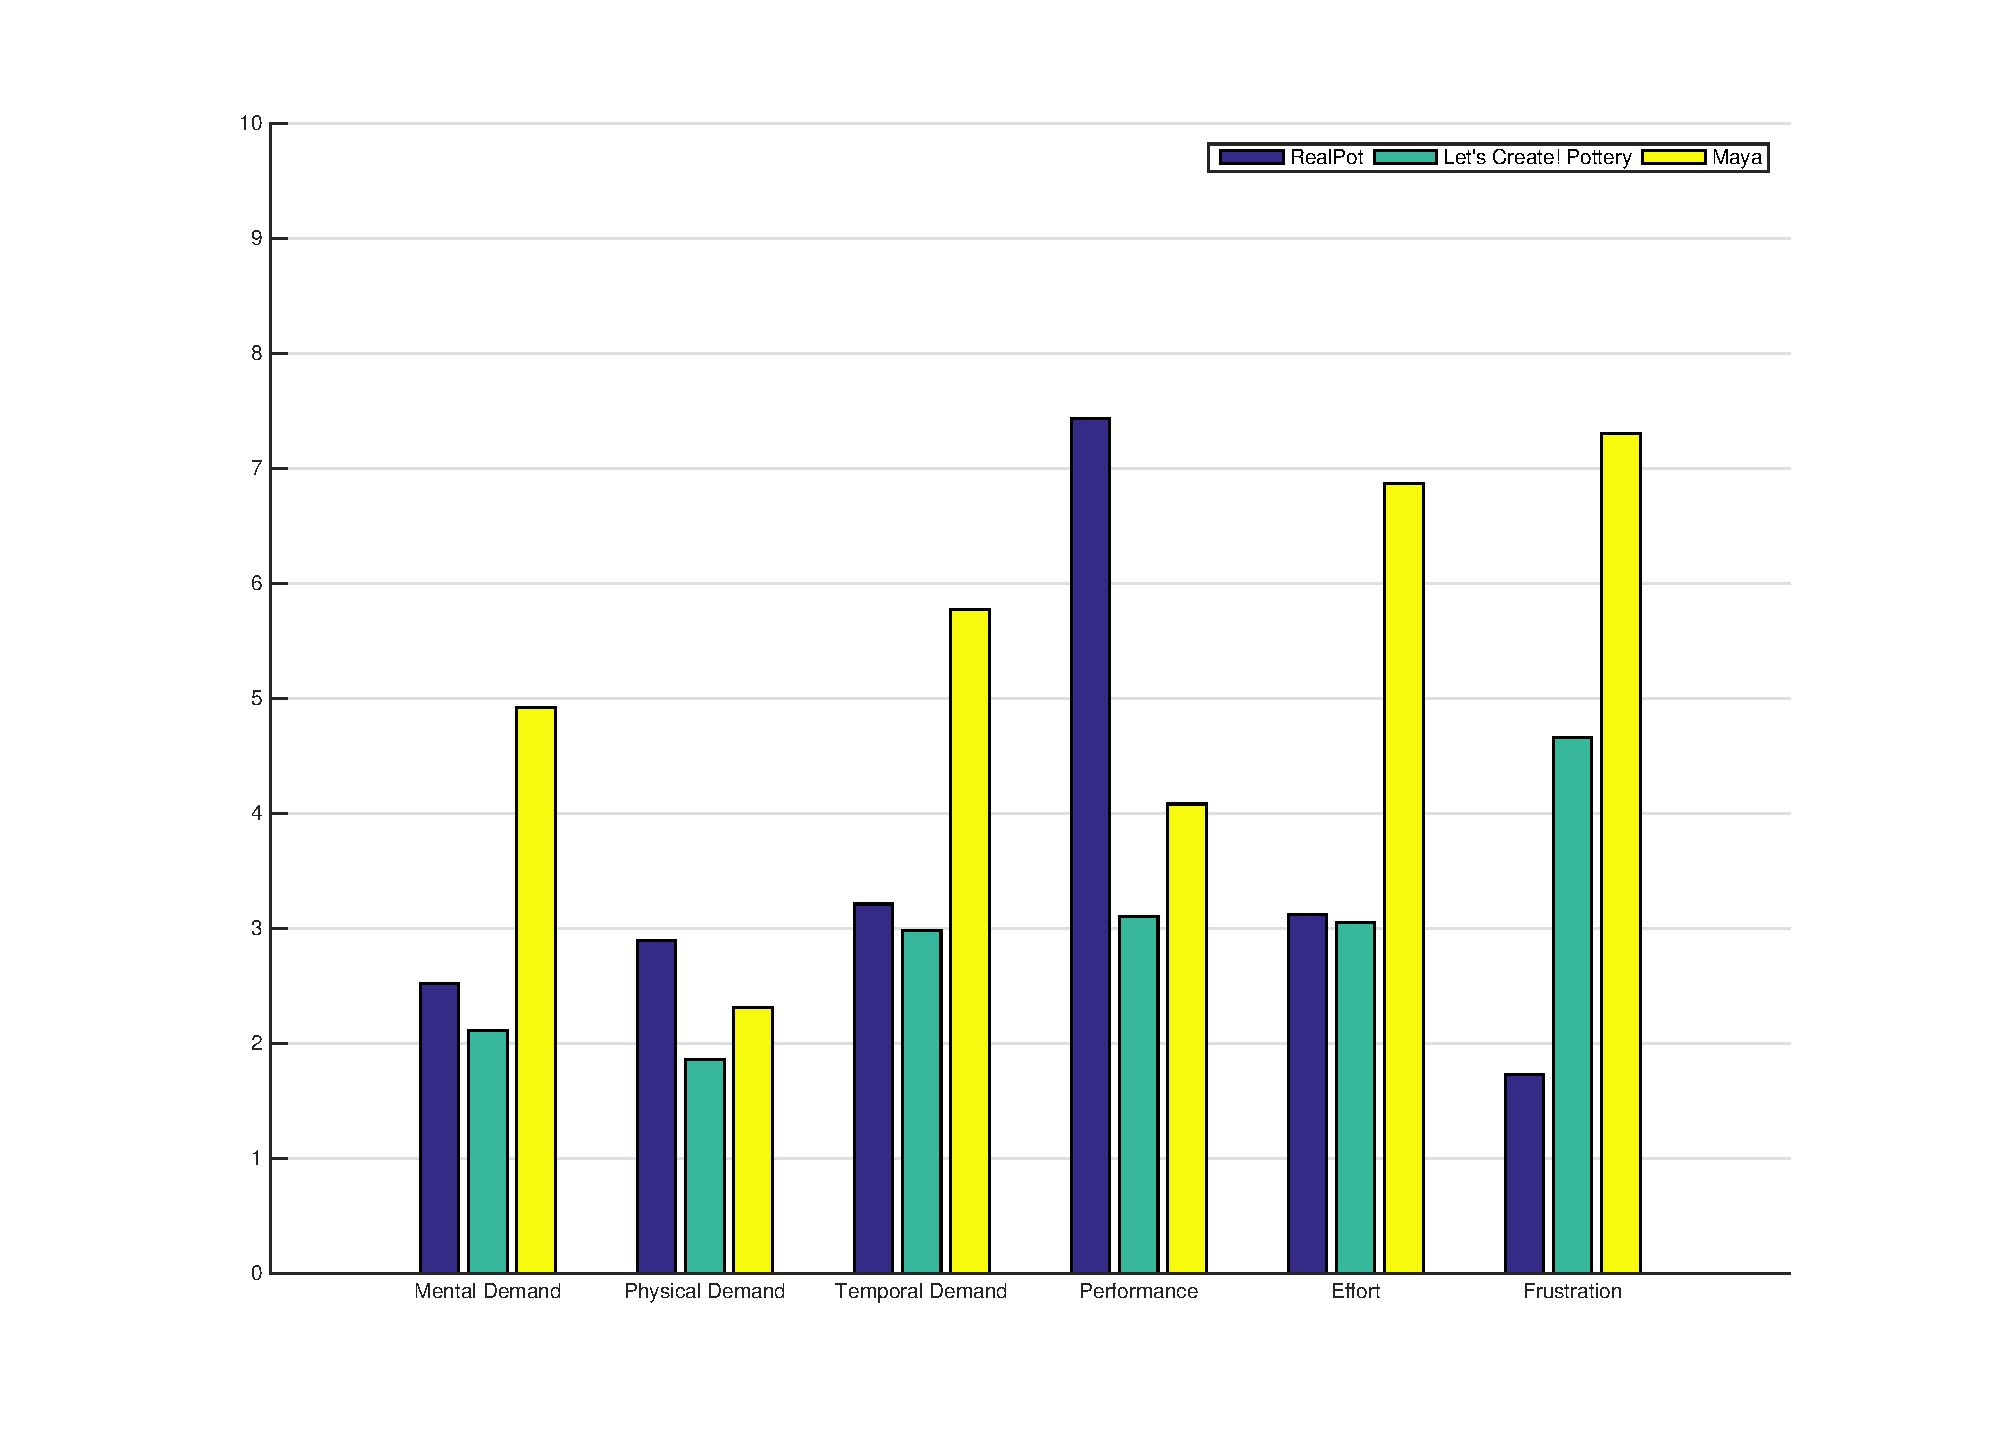
\includegraphics[width=\textwidth]{fig14}
	\caption{Results in user study 2. (a) Completion time for two compared systems. (b) Accuracy for two compared systems. (c) Presence and usability score for two compared systems.}
	\label{fig:r2}
\end{figure*}




\section{Discussions}
\label{sec:discussion}

Based on the results, our observations and user comments, we have drawn several inferences from our evaluation.

\textbf{High haptic fidelity levels enhanced productivity and user experience. }
During our user study, we observed that users seemed to have difficulty to deform the clay in the \textit{None} haptic condition.
The significant effect of haptic fidelity on completion time supported this observation, as \textit{None} was the most time-consuming condition.
In contrast, \textit{Basic} and \textit{Advanced} took significantly less time, thanks to the haptic feedback provided by the controllers.
%
The subjective usability score revealed the effectiveness of high haptic levels.
Specifically, the \textit{Advanced} condition received significantly higher usability score than the \textit{Basic} condition.
Based on the comments from participants and our observations, we attribute the high usability score to the high haptic fidelity in the \textit{Advanced} condition, which provided much realistic user experience compared with simple haptic pulses in the \textit{Basic} condition.
%
Despite the effects on completion time were significant, we found no significant effects of haptic fidelity on accuracy.
The most likely reason may be that the accuracy was calculated based on the shape data.
In the experiment, high accuracy required careful visual observation from users rather than haptic sensation.
Hence, while haptic fidelity had significant effect on completion time, the influence of haptic fidelity on accuracy was minor.

\textbf{High realism system increased performance, presence and usability. }
According to the results, our system had significantly higher presence and usability scores than DigiClay.
This is due to the fidelity level of RealPot, including first-person immersive experience and rich haptic feedbacks, was much higher than that in DigiClay.
%
The results also revealed that RealPot was significantly more accurate than DigiClay. 
From our observation and user comments, the introduction of parameter control in RealPot allowed users to create high curvature traits on the clay, which helped users to create shapes much closer to the target shape.

During user study 2, we observed that the undo/redo functionality is not used frequently as we expected.
The reason might be that each operation is an easy-to-reverse action. Unlike the actions in word processors or professional 3D modeling tools which are usually hard to reverse, if an action deformed the clay mistakenly, the user can simply deform the clay back to its original shape or to a new desired shape without using undo/redo shortcut.
In addition, undo/redo are abstract operations that are difficult to find analogies in real world, which might be another reason for not frequently used.

\textbf{Familiarity could increase user performance.}
We found a positive correlation between pottery familiarity and user performance.
%
Our results showed that users who had real-life pottery experience had significantly better performance, including completion time and accuracy.
%
We collected user feedbacks after the subjects had used our system.
In summary, subjects gave many positive feedbacks when using our system to design pottery models.
For those who had pottery experience, they spoke highly of the immersive pottery creation experience with intuitive interactions and haptic feedback that motivated them to design pottery works just like working on real clay.
According to some users who had no real-life pottery experience, they enjoyed the training process very much and would like to try real pottery someday.
We also asked their suggestions for the future features they wanted to see in RealPot.
A few subjects expressed their wishes to add coloring feature, which allows them decorate the pots with colors and patterns.

Our system still has its limitations. Although we have proposed a haptic feedback model for virtual pottery with high realism, the generated haptic effects might still be limited due to the capability of the haptic devices used in our system. Ideally, the haptic devices should be able to generate forces in 3 degrees of freedom (DOF), compared with the haptic devices used in our system, which only had 1 DOF haptic feedback.
%
Another limitation of our system is that it cannot adding handles to the pottery. We will introduce more features that allow users to modify the topology of the mesh in order to create more personalized pottery works.

\section{Conclusions}
\label{sec:conclusion}

In this paper, we have demonstrated that increased fidelity can impact usability and user performance in virtual pottery systems.
% haptic
With first-person immersive experience and realistic simulations of haptic sensation, our system improved both visual and haptic display fidelity for virtual pottery, allowing users creating a variety of pottery models in a high level of realism.
% interaction
As a training application, the proposed workflow in RealPot can help novice users getting familiar with real-life pottery effectively. In addition, the functionalities in RealPot can offer more creativity.
%
Our results have shown that realistic haptic feedback based on our proposed haptic model offers significantly better user experience, and takes much less completion time comparing to the condition without haptic feedback.
%
Compared with camera-based virtual pottery experience, our system is significantly more accurate and has higher presence and usability score.
%
For future work, a possible extension of our system is to support more features such as interactive coloring, which can enhance the artistry of user generated pottery works.

\section*{Appendix: Usability Questionnaire}

\begin{enumerate}
\item Rate how easy it was for you to shape the virtual clay (1 = extremely difficult, 7 = extremely easy).
\item Rate how natural it was for you to shape the virtual clay (1 = extremely unnatural, 7 = extremely unnatural).
\item Rate how much fun you had creating the virtual clay (1 = extremely frustrating, 7 = extremely fun).
\item Rate how creative it was for you to shape the virtual clay (1 = extremely little, 7 = extremely much).
\item Rate how tiring it was for you to shape the virtual clay (1 = extremely exhausting, 7 = not tiring at all).
\item Rate how much skills you gain from the virtual pottery training (1 = extremely little, 7 = extremely much).

\end{enumerate}

}

\begin{acknowledgements}
{\color{blue}
We thank the reviewers for their valuable feedback and comments. 
%
We also thank all the people participated in the user studies.
}
%
This work is supported by the Natural Science Foundation of China (No.~61502118), the Natural Science Foundation of Heilongjiang Province in China (No.~F2016028 and F2016009), the Fundamental Research Fund for the Central Universities in China (No.~HEUCF180602 and HEUCFM180604) and the National Science and Technology Major Project (No.~2016ZX03001023-005).
%If you'd like to thank anyone, place your comments here
%and remove the percent signs.
\end{acknowledgements}

% BibTeX users please use one of
%\bibliographystyle{spbasic}      % basic style, author-year citations
\bibliographystyle{spmpsci}      % mathematics and physical sciences
%\bibliographystyle{spphys}       % APS-like style for physics
\bibliography{pottery}   % name your BibTeX data base

% Non-BibTeX users please use
%\begin{thebibliography}{}
%
% and use \bibitem to create references. Consult the Instructions
% for authors for reference list style.
%
%\bibitem{RefJ}
% Format for Journal Reference
%Author, Article title, Journal, Volume, page numbers (year)
% Format for books
%\bibitem{RefB
%Author, Book title, page numbers. Publisher, place (year)
% etc
%\end{thebibliography}

\end{document}
% end of file template.tex

